% 来源：固定来源 PDF（2004福建文.pdf）第 1 页（印刷页 166）Q7 四选项图
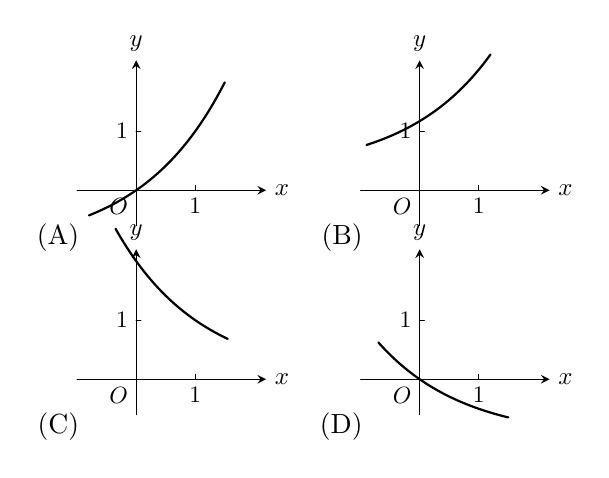
\begin{tikzpicture}[x=0.75cm, y=0.75cm, >=stealth, line cap=round, line join=round]
  \tikzset{
    axis/.style={->, thin},
    curve/.style={thick},
    tick/.style={thin}
  }

  % (A)
  \begin{scope}[shift={(0, 3.2)}]
    \draw[axis] (-1.0, 0) -- (2.2, 0) node[right, scale=0.9] {$x$};
    \draw[axis] (0, -0.6) -- (0, 2.2) node[above, scale=0.9] {$y$};
    \node[below left, scale=0.85] at (0, 0) {$O$};
    \draw[tick] (1, 0) -- (1, 0.08);
    \node[below, scale=0.85] at (1, 0) {$1$};
    \draw[tick] (0, 1) -- (0.08, 1);
    \node[left, scale=0.85] at (0, 1) {$1$};
    \draw[curve, domain=-0.8:1.5, samples=50] plot (\x, {2^(\x) - 1});
    \node[below left] at (-0.8, -0.4) {(A)};
  \end{scope}

  % (B)
  \begin{scope}[shift={(4.8, 3.2)}]
    \draw[axis] (-1.0, 0) -- (2.2, 0) node[right, scale=0.9] {$x$};
    \draw[axis] (0, -0.6) -- (0, 2.2) node[above, scale=0.9] {$y$};
    \node[below left, scale=0.85] at (0, 0) {$O$};
    \draw[tick] (1, 0) -- (1, 0.08);
    \node[below, scale=0.85] at (1, 0) {$1$};
    \draw[tick] (0, 1) -- (0.08, 1);
    \node[left, scale=0.85] at (0, 1) {$1$};
    \draw[curve, domain=-0.9:1.2, samples=50] plot (\x, {2^(\x - 0.2) + 0.3});
    \node[below left] at (-0.8, -0.4) {(B)};
  \end{scope}

  % (C)
  \begin{scope}[shift={(0, 0)}]
    \draw[axis] (-1.0, 0) -- (2.2, 0) node[right, scale=0.9] {$x$};
    \draw[axis] (0, -0.6) -- (0, 2.2) node[above, scale=0.9] {$y$};
    \node[below left, scale=0.85] at (0, 0) {$O$};
    \draw[tick] (1, 0) -- (1, 0.08);
    \node[below, scale=0.85] at (1, 0) {$1$};
    \draw[tick] (0, 1) -- (0.08, 1);
    \node[left, scale=0.85] at (0, 1) {$1$};
    \draw[curve, domain=-0.35:1.55, samples=50] plot (\x, {2^(1 - \x)});
    \node[below left] at (-0.8, -0.4) {(C)};
  \end{scope}

  % (D)
  \begin{scope}[shift={(4.8, 0)}]
    \draw[axis] (-1.0, 0) -- (2.2, 0) node[right, scale=0.9] {$x$};
    \draw[axis] (0, -0.6) -- (0, 2.2) node[above, scale=0.9] {$y$};
    \node[below left, scale=0.85] at (0, 0) {$O$};
    \draw[tick] (1, 0) -- (1, 0.08);
    \node[below, scale=0.85] at (1, 0) {$1$};
    \draw[tick] (0, 1) -- (0.08, 1);
    \node[left, scale=0.85] at (0, 1) {$1$};
    \draw[curve, domain=-0.7:1.5, samples=50] plot (\x, {2^(-\x) - 1});
    \node[below left] at (-0.8, -0.4) {(D)};
  \end{scope}
\end{tikzpicture}
